\documentclass{article}
\usepackage{graphicx}
\usepackage[margin=1.5cm]{geometry}
\usepackage{amsmath}

\begin{document}

\title{Tuesday Reading Assessment: Chapter 4}
\author{Prof. Jordan C. Hanson}

\maketitle

\section{Boolean Algebra}

\begin{enumerate}
\item Write the truth table for the following boolean expression:
\begin{equation}
\bar{X} \bar{Y} \bar{Z} + \bar{X}\bar{Y}Z + XY\bar{Z} + X\bar{Y}Z + \bar{X}YZ
\end{equation}
\vspace{5cm}
\end{enumerate}

\section{Logic Circuits and Boolean Algebra}

\begin{enumerate}
\item Write the boolean expression for the circuit in Fig. \ref{fig:gates1}.
\begin{figure}[ht]
\centering
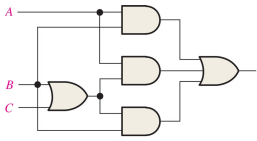
\includegraphics[width=0.35\textwidth]{gates1.png}
\caption{\label{fig:gates1} What is the logical expression for the output?}
\end{figure}
\end{enumerate}

\end{document}
